%!TEX root = thesis.tex

\section{Reproducibility self-assessment}
\label{sec:reproducibility}

\begin{figure}[h]
  \centering
  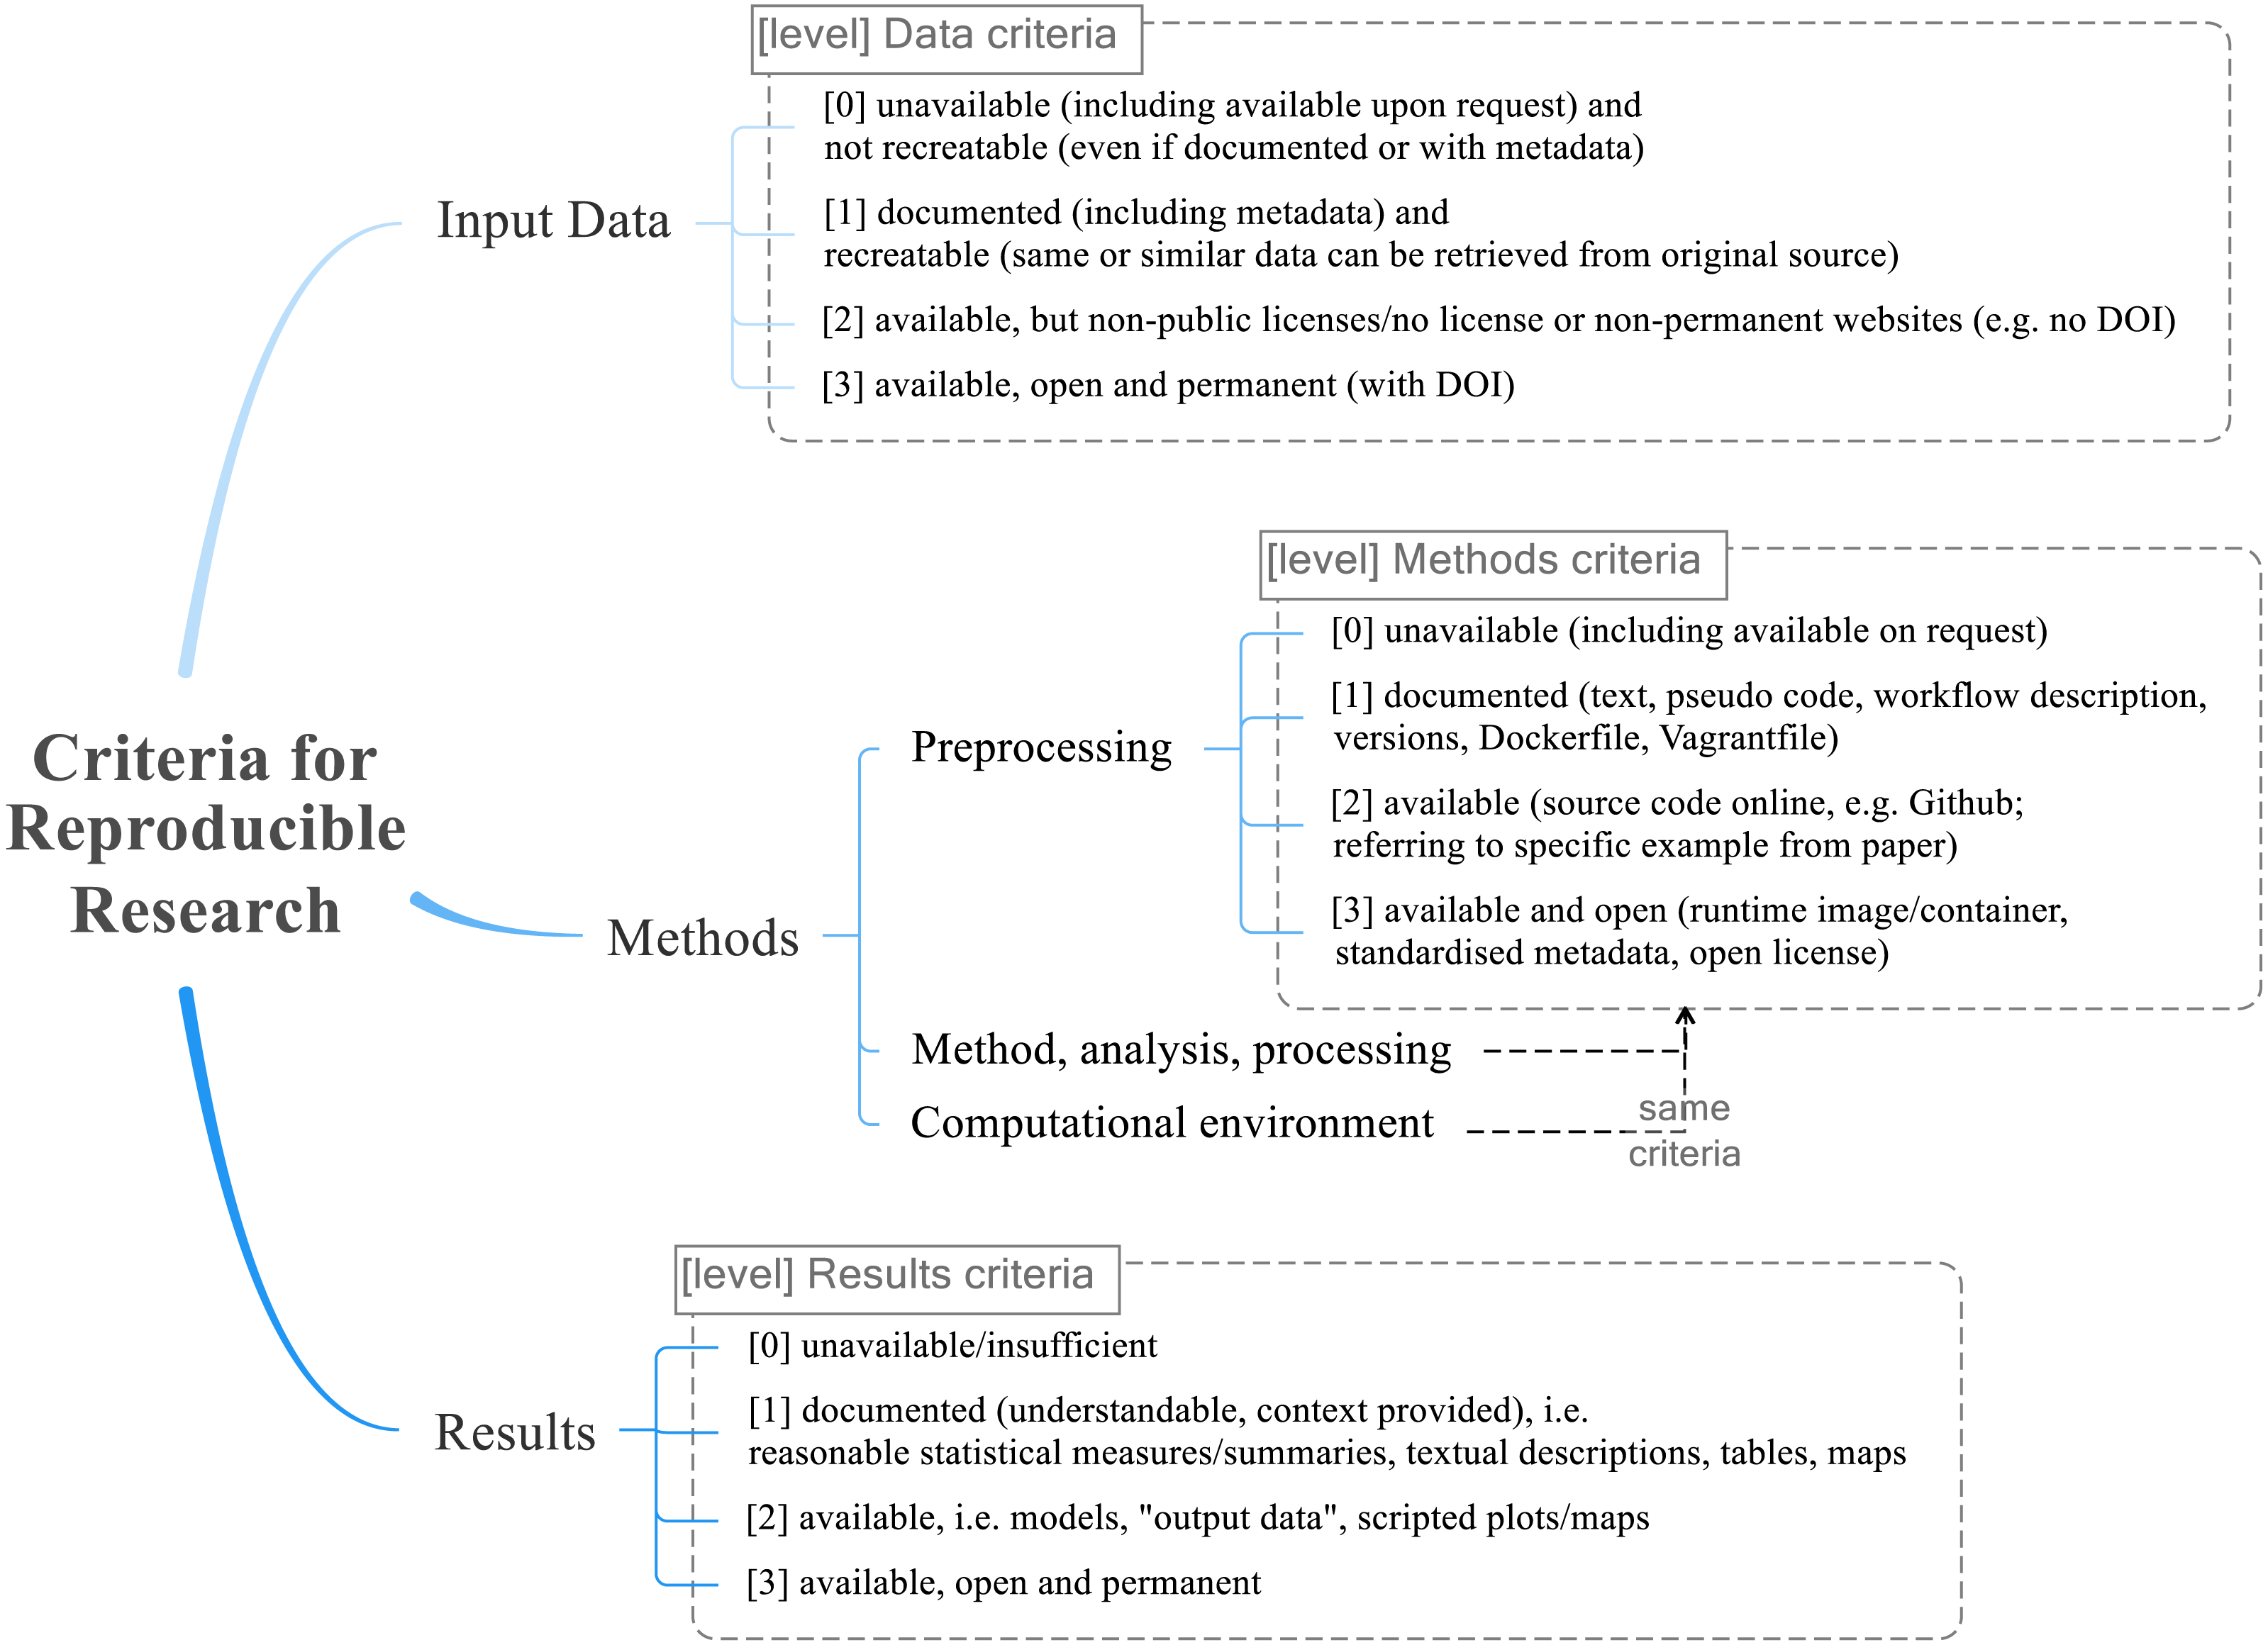
\includegraphics[width=0.9\linewidth]{figs/reproducibility_criteria.png}
  \caption{Reproducibility criteria to be assessed.}
\label{fig:reproducibility_criteria}
\end{figure}


Preliminary reproducibility self-assessment grades on a scale of 1 to 3:

\begin{enumerate}
  \item input data - \textbf{Grade = 3}
  \item preprocessing - \textbf{Grade = 2}
  \item methods - \textbf{Grade = 3}
  \item computational environment - \textbf{Grade = 3}
  \item results - \textbf{Grade = 2}
\end{enumerate}

\textit{[To be finalised for the final (P5) version of this report.]}

\section{Self-reflection} 

\textit{[To be produced for the final (P5) version of this report.]}